% BOTH

Hauptziel der Arbeit war es die Komponenten gut zu vermessen und ihre Leistung zu verifizieren.

\subsubsection*{Setup}

\subsubsection*{Erste Messungen}

Mit einer ersten bestückten Leiterplatte wurden daher mit dem Oszilloskop erste Messungten durchgeführt, welche eine generelle Funktionstüchtigkeit bezeugten, welche aber gar nicht zufriedenstellend war.

\begin{figure}[ht]
\begin{center}
    \includegraphics[width=0.9\textwidth]{data/images/messungen/erste_messung}
    \caption{Erste Messungen des Gesamtsystems. Inkorrekt terminiert. Mit Oszilloskop gemessen.}
    \label{fig:messungen_erste}
\end{center}
\end{figure}

Diese Kurve sieht wahnsinnig unschön aus. Gerade bei den Peaks gibt es fiese Ausreisser. Und was ebenfalls nicht zu vernachlässigen ist, sind die 180 Grad Phasenverschiebung.
Auch sieht man hier, dass der dass der Input des Funktionsgenerators ziemlich viel Rauschen hat, welches sich auch in Grafik \ref{fig:messungen_zweite} zeigt.
Dort sieht man gut, dass der Input ziemlich rauscht. Deswegen haben wir versucht N und P voneinander zu subtrahieren. Und so das Rauschen zu eliminieren. Dies hat sogar relativ gut geklappt. Dies ist natürlich nicht ganz sauber, ging aber für eine erste Verifikation sehr gut.

\begin{figure}[ht]
\begin{center}
    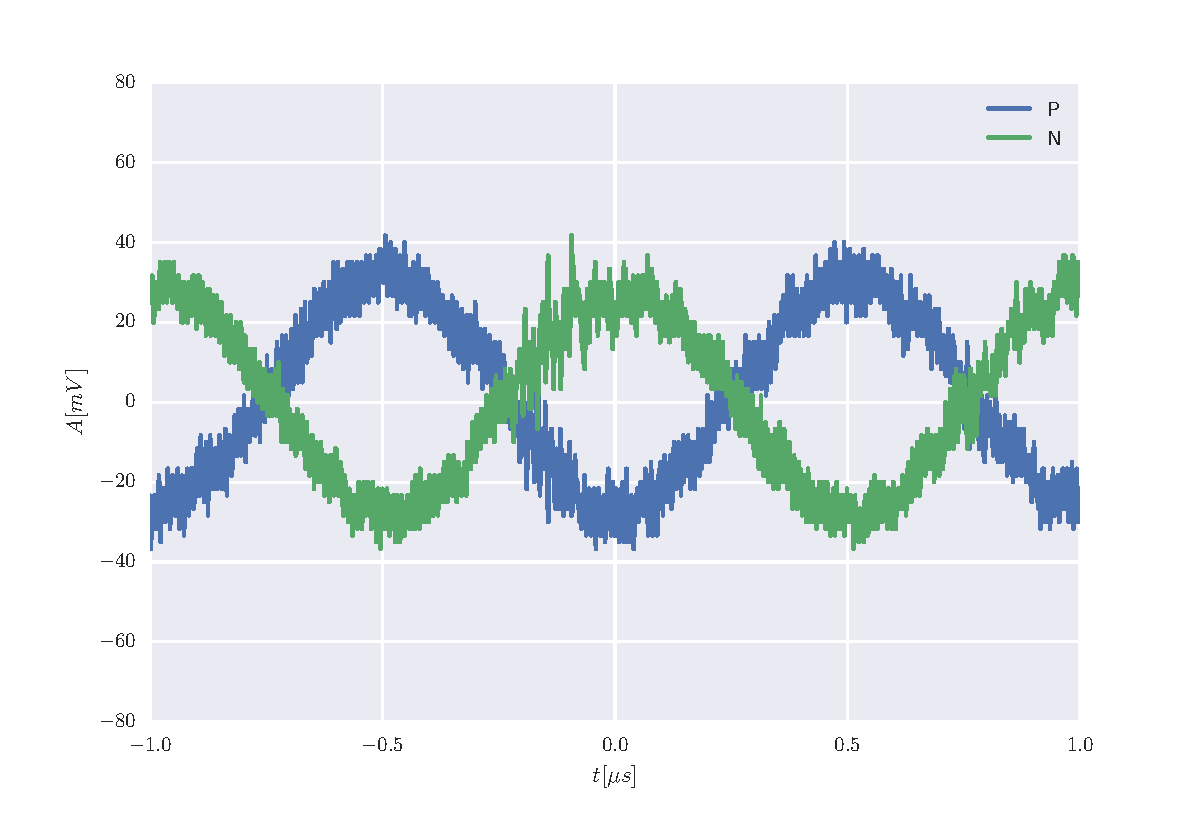
\includegraphics[width=0.9\textwidth]{data/images/messungen/zweite_messung_NP}
    \includegraphics[width=0.9\textwidth]{data/images/messungen/zweite_messung_INOUT}
    \caption{Erste Messungen des Gesamtsystems. Inkorrekt terminiert. Mit Oszilloskop gemessen.}
    \label{fig:messungen_zweite}
\end{center}
\end{figure}

Bei diesen Messungen war jedoch das DUT nicht korrekt terminiert. Dies war einer der Knackpunkte zum Anfang. Es war uns bekannt, dass Dinge in diesem Gebiet korrekt terminiert werden müssen. Wenn das DUT nicht korrekt belastet wird können ungewollte Effekte auftreten. Deswegen sind diese ersten Messungen mit Vorsicht zu geniessen und dürfen nur als Anhaltspunkt und nicht als exakte Messung genommen werden.

Eigentlich wären zur korrekten Terminierung und Umwandlung in ein single-ended Signal, wie im Abschnitt \ref{Leiterplattendesign} beschrieben, Baluns vorgesehen. Diese sind jedoch relativ schwer zu kriegen und sind dann relativ teuer. Deswegen wurde eine günstigere Lösung gesucht. Diese wurde in der Schaltung dargestellt in \ref{fig:terminator} gefunden.

\begin{figure}[ht]
\begin{center}
    \begin{circuitikz}
        \draw[dashed] node[tground]{}
        to[V,v=$U_q$] (0,2)
        to[short] (1,2);

        \draw (1,2)
        node[ocirc]{}
        to[short] (2,2)
        to[R=$237\Omega$] (4,2)
        to[short] (6, 2)
        node[ocirc]{};

        \draw (5,2)
        to[R=$28\Omega$] (5,0)
        node[tground]{};

        \draw[dashed] (6, 2)
        to[short] (7, 2)
        to[R=$25\Omega$] (9,2)
        to[short] (9, 0)
        node[tground]{};

        % Lower side

        \draw[dashed] (0, 0)
        to [V,v=$U_q$] (0,-2)
        to[short] (1,-2);

        \draw (1,-2)
        node[ocirc]{}
        to[short] (2,-2)
        to[R=$250\Omega$] (4,-2)
        to[short] (5, -2)
        to[short] (5, 0);

        \draw[dashed] (-1, 4)
        to[short] (1, 4)
        to[short] (1, -4)
        to[short] (-1, -4);

        \draw[dashed] (12, 4)
        to[short] (6, 4)
        to[short] (6, -4)
        to[short] (12, -4);

    \end{circuitikz}
    \caption{Terminierung des AD8331 zur Messung mit single-ended Geräten die 50 Ohm-Terminierung haben.}
    \label{fig:terminator}
\end{center}
\end{figure}